\documentclass[10pt]{beamer}
%\documentclass[10pt]{beamer}
\usetheme[
%%% option passed to the outer theme
%    progressstyle=fixedCircCnt,   % fixedCircCnt, movingCircCnt (moving is deault)
]{Feather}

%\setbeamertemplate{blocks}[rounded][shadow=true]
%\setbeamertemplate{background canvas}[vertical shading][bottom=white,top=structure.fg!25]
%\setbeamertemplate{sidebar canvas left}[horizontal shading][left=white!40!black,right=black]


\usepackage[T2A,T1]{fontenc}
\usepackage[utf8]{inputenc}
\usepackage[russian,english]{babel}

 \usepackage{helvet}
 \usepackage{graphicx}
 \usepackage{wrapfig}
 \usepackage{listings}

 \usepackage{ragged2e}  % `\justifying` text
 \usepackage{booktabs}  % Tables
 \usepackage{tabularx}
 \usepackage{tikz}      % Diagrams
 \usetikzlibrary{calc, shapes, backgrounds}
 \usepackage{amsmath, amssymb}
 \usepackage{url}       % `\url`s

 \usepackage{color}

 \definecolor{mygreen}{rgb}{0,0.6,0}
 \definecolor{mygray}{rgb}{0.5,0.5,0.5}
 \definecolor{mymauve}{rgb}{0.58,0,0.82}
 \definecolor{mybgray}{HTML}{EDECF0}

 \lstset{ %
	 backgroundcolor=\color{mybgray},   % choose the background color; you must add \usepackage{color} or \usepackage{xcolor}
      commentstyle=\color{mygreen},    % comment style
      extendedchars=true,              % lets you use non-ASCII characters; for 8-bits encodings only, does not work with UTF-8
     keywordstyle=\color{blue},       % keyword style
     language=Python,                 % the language of the code
     rulecolor=\color{black},         % if not set, the frame-color may be changed on
     stringstyle=\color{mymauve},     % string literal style
     numbers=left,     
}

 \newcommand{\chref}[2]{
 	\href{#1}{{\usebeamercolor[bg]{Feather}#2}}
 }

 \author
 {    Aleksei Buziuma \\
 	EPAM Systems, Low Level Programming Department
 	{\ttfamily buzuma.leha@gmail.com}
 }
 
 \subject{Python language}

 \institute[]
 {
 	Belorussian State University Of Informatics and Radio-electronics.\\
 	Faculty of computer system and networks.\\
 	Electronic Computing Machines Department.\\
 }

 \date{\today}


\title[Why you need to learn Python?] % [] is optional - is placed on the bottom of the sidebar on every slide
{
	\textbf{Why do you need to learn Python?}
}

\begin{document}
	
{\1% % this is the name of the PDF file for the background
	\begin{frame}[plain,noframenumbering] 
		\titlepage
	\end{frame}
}

% Show table of content	
%\begin{frame}{Content}{}
%\end{frame}
		
%-------------------------------------------------------
\section{Introduction}
%-------------------------------------------------------

%-------------------------------------------------------
\subsection{What is Python?}
%-------------------------------------------------------


% ********************** Slide 2 ***********************
\begin{frame}{Problem of improper use.}
%-------------------------------------------------------
\begin{center}
	\LARGE Why do I need a Scala? \\I'am JS programmer!
\end{center}
\end{frame}
% ******************************************************

% ********************** Slide 2 ***********************
\begin{frame}{Introduction}{Problem of improper use.}
	%-------------------------------------------------------
	\begin{center}
		\large{I can solve any problem with my programming language!}
		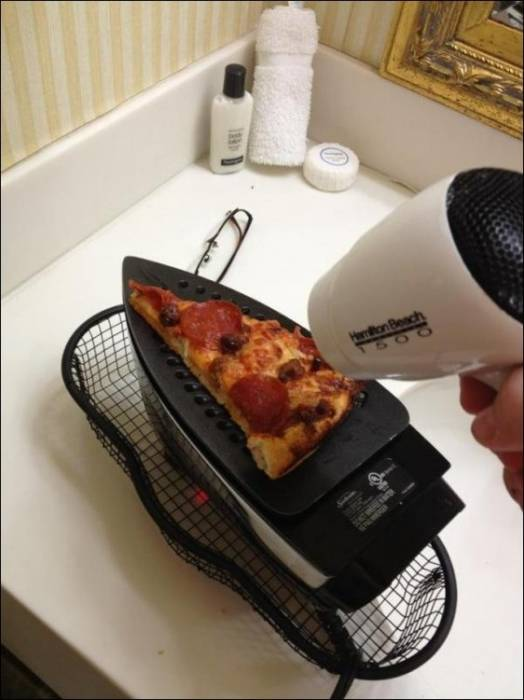
\includegraphics[width=0.4\textwidth]{pictures/improper.jpg}
	\end{center}
\end{frame}
% ******************************************************

% ********************** Slide 2 ***********************
\begin{frame}{Introduction}{What is Python?}
%-------------------------------------------------------
	\begin{center}
		
\includegraphics[width=0.6\textwidth]{pictures/python.png}
	\end{center}
\end{frame}
% ******************************************************

% ********************** Slide 3 ***********************
\begin{frame}{Introduction}{What is Python?}
%-------------------------------------------------------
	\begin{block}{Python}
		Python is an interpreted, object-oriented, high-level programming language with dynamic semantics.  This is a general-purpose language that can be equally well developed system applications with a graphical interface, command line utilities, scientific applications, games, applications for the Web, and much more.	
	\end{block}
\end{frame}
% *****************************************************

%-------------------------------------------------------
\subsection{Dinamic vs Static}
%-------------------------------------------------------
% ********************** Slide 5 ***********************
\begin{frame}[fragile]{Introduction}{Dinamic vs Static}
	\begin{center}
		\LARGE What is dynamic / static typing? \\
		\pause
		\LARGE What is strong / weak typing? \\
		\pause 
		\LARGE What is explicit / implicit typing
	\end{center}
\end{frame}

% ********************** Slide 4 ***********************
\begin{frame}{Introduction}{What is Python?}
%-------------------------------------------------------
	\begin{center}
		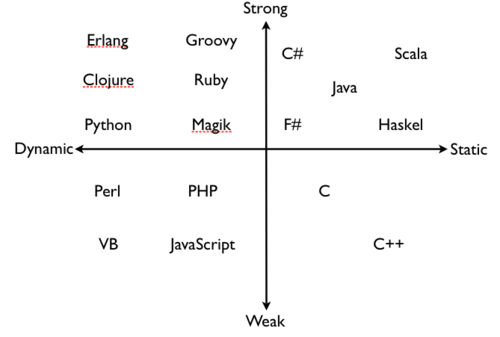
\includegraphics[width=0.9\textwidth]{pictures/1.png}
	\end{center}
\end{frame}
% ******************************************************



%-------------------------------------------------------
\subsection{Dinamic vs Static}
%-------------------------------------------------------

% ********************** Slide 5 ***********************
\begin{frame}[fragile]{Introduction}{Dinamic vs Static}
%-------------------------------------------------------
\begin{center}
\begin{block}{Dinamic -- Python (JavaScript, Ruby)}
			
\begin{lstlisting}[language=Python]
>>> string = "string"
>>> type(string)
<class 'str'>

>>> number = 42
>>> type(number)
<class 'int'>

\end{lstlisting}
\end{block}
		
\pause
		
\begin{block}{Static -- Java (C, C++, C\#)}
			
\begin{lstlisting}[language=Java]
int i = 42;
String greeting = "Hello world!";
\end{lstlisting}

\end{block}

\end{center}
\end{frame}
% ******************************************************

%-------------------------------------------------------
\subsection{Strong vs Weak}
%-------------------------------------------------------

% ********************** Slide 9 ***********************
\begin{frame}[fragile]{Introduction}{Strong vs Weak}
%-------------------------------------------------------
	
\begin{center}
		
\begin{block}{Strong -- Python}
\begin{lstlisting}[language=Python]
>>> print 13 + "13"
TypeError
>>> print [] + {}
TypeError
\end{lstlisting}
\end{block}
		
\pause
		
\begin{block}{Strong -- Ruby}
\begin{lstlisting}[language=Ruby]
irb(main)> 42 + "42"
TypeError
irb(main)> [] + {}
TypeError
\end{lstlisting}
\end{block}
		
\end{center}
	
\end{frame}
% ******************************************************

% ********************** Slide 6 ***********************
\begin{frame}[fragile]{Introduction}{Let's talk about JavaScript!}
%-------------------------------------------------------
\begin{center}
	
\begin{block}{Weak -- JavaScript}
	
\begin{lstlisting}
>>> [] + []  
>>>

>>> [] + {} 
[object Object]

>>> {} + []  
0

>>> {} + {}  
NaN
\end{lstlisting}


\end{block}

\end{center}

\end{frame}
% ******************************************************


% ********************** Slide 7 ***********************
\begin{frame}[fragile]{Introduction}{Let's talk about JavaScript!}
%-------------------------------------------------------
\begin{center}
		
\begin{block}{Weak -- JavaScript}
			
\begin{lstlisting}
> '5' - 3
2
> '5' + 3
'53'
>'foo' + + 'foo'
'fooNaN'
>'5' + - '2'
'5-2'
> var x = 3;
>'5' + x - x
50
>'5' - x + x
5
\end{lstlisting}
			
			
\end{block}
		
\end{center}
	
\end{frame}
% ******************************************************


% ********************** Slide 8 ***********************
\begin{frame}{Introduction}{Typing}
%-------------------------------------------------------
	\begin{center}
		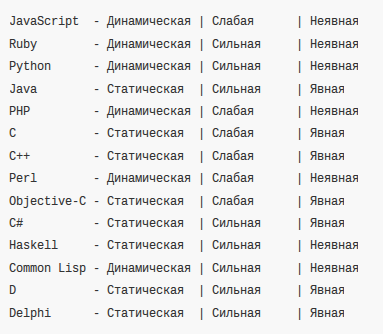
\includegraphics[width=0.75\textwidth]{pictures/typing.png}
	\end{center}
\end{frame}
% ******************************************************


% ********************** Slide 8 ***********************
\begin{frame}{Introduction}{WAAAAAT?}
%-------------------------------------------------------
	\begin{center}
		
\includegraphics[width=0.9\textwidth]{pictures/wat.jpg}
	\end{center}
\end{frame}
% ******************************************************


% ********************** Slide 2 ***********************
\begin{frame}{Introduction}{Let's talk about JavaScript!}
%-------------------------------------------------------
\begin{center}
	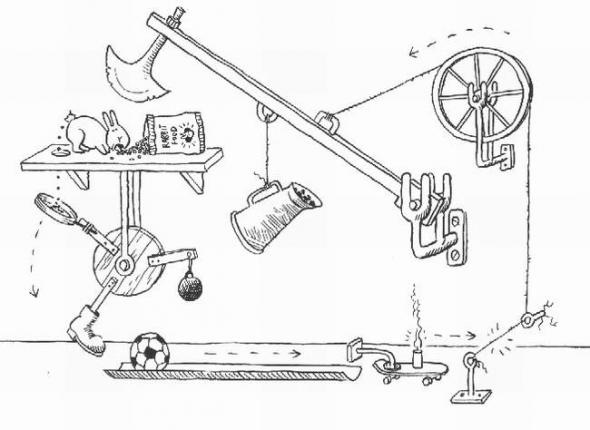
\includegraphics[width=0.9\textwidth]{pictures/shot.jpg}
\end{center}
\end{frame}
% ******************************************************

% ********************** Slide 2 ***********************
\begin{frame}{Introduction}{Why JS is terrible?}
%-------------------------------------------------------
\begin{center}
	\begin{block}{Why JS is terrible?}
		\begin{itemize}
			\item \url{https://whydoesitsuck.com/why-does-javascript-suck/}
			\pause 
			
			\item \url{http://live.julik.nl/2013/05/javascript-is-shit}
			\pause 
			
			\item \url{http://www.boronine.com/2012/12/14/Why-JavaScript-Still-Sucks/}
			\pause
			
			\item \url{https://simpleprogrammer.com/2013/05/06/why-javascript-is-doomed/}
			\pause
			
			\item \url{https://kaushalsubedi.com/blog/2014/10/15/node-js-sucks-heres-why/}
			
		\end{itemize}
	\end{block}
\end{center}|

\end{frame}


% ********************** Slide 2 ***********************
\begin{frame}{Introduction}{Links}
%-------------------------------------------------------
\begin{center}
	\Large{Nothing is perfect} 
	\url{https://wiki.theory.org/YourLanguageSucks/}
\end{center}|
\end{frame}

%-------------------------------------------------------
\subsection{History of Python}
%-------------------------------------------------------

\begin{frame}{Introduction}{History of Python}
%-------------------------------------------------------
	\begin{tikzpicture}[overlay,remember picture]
	\node[anchor=south east,xshift=-10pt,yshift=20pt]
	at (current page.south east) {
		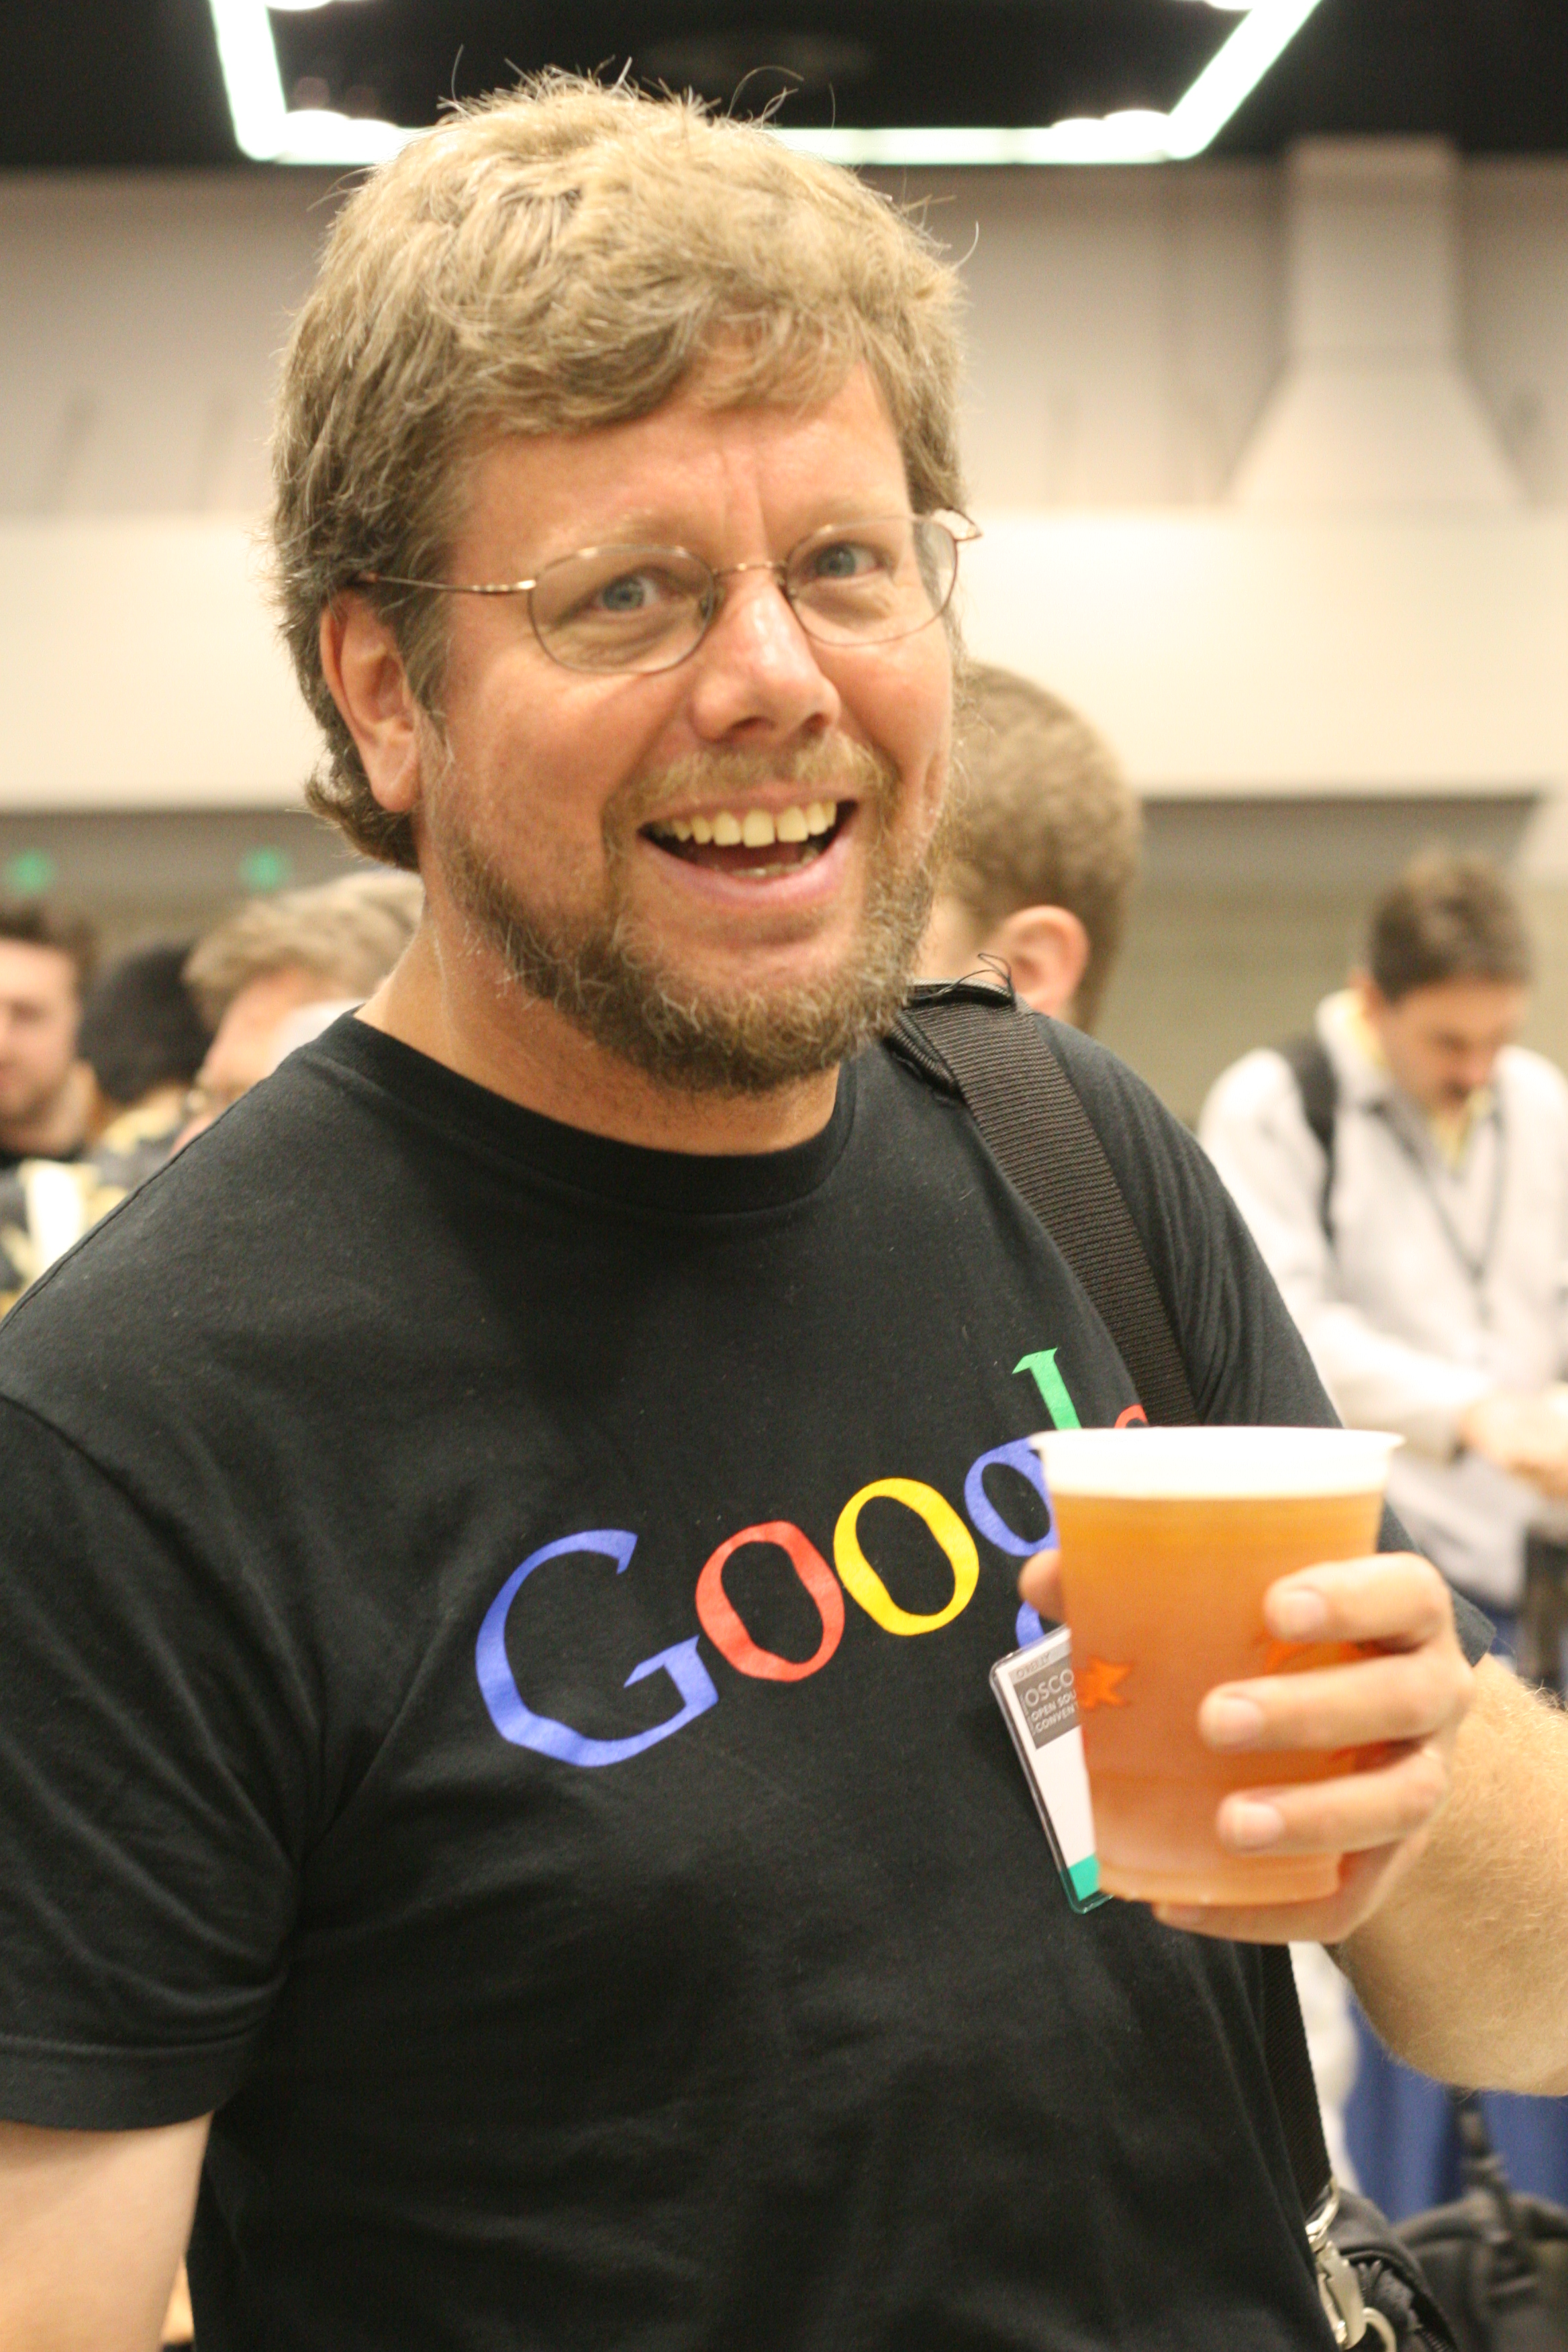
\includegraphics[width=0.4\textwidth]{pictures/1.jpg}
	};
	\end{tikzpicture}
	
	Guido van Rossum is a Dutch computer \\ 
	programmer who is best known as the \\
	author of the Python programming \\
	language. In the Python community, \\
	Van Rossum is known as a "Benevolent \\
	Dictator For Life" (BDFL), meaning \\
	that he continues to oversee the Python\\
	development process, making decisions \\
	where necessary.He was employed by \\
	Google from 2005 until 7 December 2012,\\
	where he spent half his time developing \\
	the Python language. In January 2013, \\
	Van Rossum started working for Dropbox.
\end{frame}
%-------------------------------------------------------

%-------------------------------------------------------
\subsection{Versions}
\begin{frame}{Introduction}{Versions}
	%-------------------------------------------------------
	\begin{block}{Implementation started | December 1989}
		\begin{itemize}
			\item First appeared - 20 February 1991, 25 years ago
		\end{itemize}
	\end{block}	
		
	\begin{block}{Python 1.0 | January 1994}
		\begin{itemize}
			\item Python 1.6 - September 5, 2000
		\end{itemize}
	\end{block}	
	
	\begin{block}{Python 2.0 | October 16, 2000}
		\begin{itemize}
			\item Python 2.7 - July 3, 2010
		\end{itemize}
	\end{block}
	
	\begin{block}{Python 3.0 | December 3, 2008}
		\begin{itemize}
			\item Python 3.5 - September 13, 2015
		\end{itemize}
	\end{block}
\end{frame}
%-------------------------------------------------------


% ********************** Slide 10 ***********************
\begin{frame}{Introduction}{Pros and cons}
%-------------------------------------------------------
	\begin{itemize}
		\item Pross
		\begin{itemize}
			\item Easy to learn
			\item Cross-platform
			\item Community
			\item Open License
			\item Efficiency
			\item Simplicity
			\item Batteries
		\end{itemize}
		
		
		\item Cons
		\begin{itemize}
			\item GIL (???)
			\item Perfomance (???)
		\end{itemize}
		
	\end{itemize}	
\end{frame}
%-------------------------------------------------------


% ********************** Slide 11 ***********************
\begin{frame}{Introduction}{Stackoverflow statistic}
%-------------------------------------------------------
	\begin{center}
		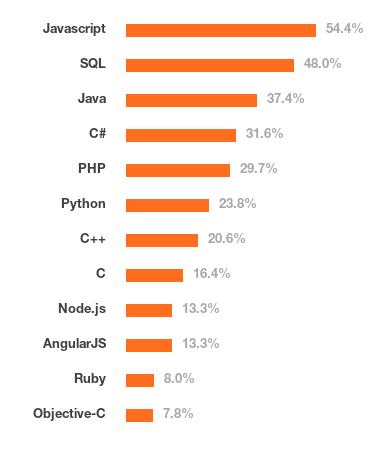
\includegraphics[width=0.6\textwidth]{pictures/stackoverflow.jpg}
	\end{center}
\end{frame}
% ******************************************************

% ********************** Slide 12 **********************
\begin{frame}{Introduction}{RedMonk statistic}
%-------------------------------------------------------
	\begin{center}
		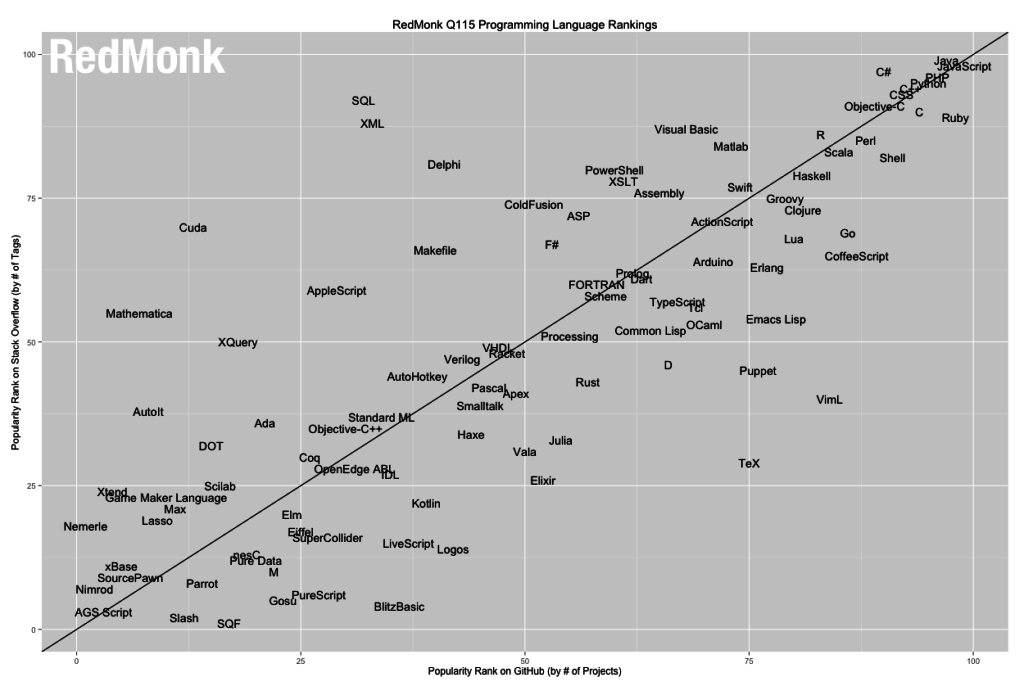
\includegraphics[width=1\textwidth]{pictures/red_monk.png}
	\end{center}
\end{frame}
% ******************************************************

%-------------------------------------------------------
\subsection{Where Python can be used?}
%-------------------------------------------------------

% ********************** Slide 13 **********************
\begin{frame}{Introduction}{Where Python can be used?}
%-------------------------------------------------------

\begin{block}{Science}
	\begin{itemize}	
		\item NumPy - a numerical Python library (a bedrock library for anything to do with matrices)
		
		\item Pandas - a library for data analysis, similar to R’s data frames or an Excel spreadsheet, built on scipy and numpy
		
		\item Scikit-learn - rapidly turning into the default machine learning library, built on scipy
		
		\item Biopython - a bioinformatics library similar to bioperl
		
		\item SymPy - a symbolic manipulation package, written in pure Python.
	\end{itemize}
	
\end{block}
\end{frame}
% ******************************************************

% ********************** Slide 14 **********************
\begin{frame}{Introduction}{Where Python can be used?}
%-------------------------------------------------------
	
	\begin{block}{Web}
		\begin{itemize}
			\item Django
			
			\item Pyramid
			
			\item Bottle
			
			\item Flask
			
			\item Tornado
		\end{itemize}
		
	\end{block}
\end{frame}
% ******************************************************

% ********************** Slide 14 **********************
\begin{frame}{Introduction}{Where Python can be used?}
	%-------------------------------------------------------
	
	\begin{block}{High Perfomance Python}
		\begin{itemize}
			\item Cython
			
			\item Numba
			
			\item Pythran
			
			\item PyPy
			
			\item Shed Skin
		\end{itemize}
		
	\end{block}
\end{frame}
% ******************************************************

% ********************** Slide 14 **********************
\begin{frame}{Introduction}{Where Python can be used?}
%-------------------------------------------------------
	
	\begin{block}{GUI applications}
		\begin{itemize}
			\item PyQT
			
			\item PyGTK
			
			\item Kivy
			
			\item wxWidgets
	
		\end{itemize}
		
	\end{block}
\end{frame}
% ******************************************************


% ********************** Slide 14 **********************
\begin{frame}[fragile]{Introduction}{IDE}
	%-------------------------------------------------------
	
	\begin{block}{IDE}
		\begin{itemize}
			
			\item PyCharm
			
			\item Sublime Text
			
			\item Atom
			
			\item Vim
			
			\item Jupyter
			
			\item ipython, bpython
		\end{itemize}
	\end{block}	
	
\end{frame}
%-------------------------------------------------------

% ********************** Slide 14 **********************
\begin{frame}{Introduction}{What is written on Python?}
%-------------------------------------------------------
	\begin{center}
		\Huge What is written on Python?
	\end{center}
\end{frame}
% ******************************************************

% ********************** Slide 14 **********************
\begin{frame}{Introduction}{What is written on Python?}
	%-------------------------------------------------------
	\begin{center}
		
\includegraphics[width=0.9\textwidth]{pictures/bit_torrent.png}
		\large{\\BitTorrent, original client, along with several derivatives}
	\end{center}
\end{frame}
% ******************************************************

% ********************** Slide 14 **********************
\begin{frame}{Introduction}{What is written on Python?}
	%-------------------------------------------------------
	\begin{center}
		
\includegraphics[width=1\textwidth]{pictures/dropbox.png}
		\large{\\Dropbox, a web-based file hosting service}
	\end{center}
\end{frame}
% ******************************************************

% ********************** Slide 14 **********************
\begin{frame}{Introduction}{What is written on Python?}
	%-------------------------------------------------------
	\begin{center}
		
\includegraphics[width=1\textwidth]{pictures/open_stack.png}
		\large{\\OpenStack, a cloud computing IaaS platform}
	\end{center}
\end{frame}
% ******************************************************

% ********************** Slide 14 **********************
\begin{frame}{Introduction}{What is written on Python?}
	%-------------------------------------------------------
	\begin{center}
		
\includegraphics[width=1\textwidth]{pictures/google.png}
		\\"Python has been an important part of Google since the beginning, and remains so as the system grows and evolves. Today dozens of Google engineers use Python, and we're looking for more people with skills in this language." said Peter Norvig, director of search quality at Google, Inc.
	\end{center}
\end{frame}
% ******************************************************

% ********************** Slide 14 **********************
\begin{frame}{Introduction}{What is written on Python?}
	%-------------------------------------------------------
	\begin{center}
		
\includegraphics[width=1\textwidth]{pictures/world_of_tanks.png}
		\large{\\World of Tanks uses Python for most of its tasks}
	\end{center}
\end{frame}
% ******************************************************

% ********************** Slide 14 **********************
\begin{frame}{Introduction}{What is written on Python?}
	%-------------------------------------------------------
	\begin{center}
		
\includegraphics[width=0.6\textwidth]{pictures/batl2.jpg}
		\large{\\Battlefield 2 uses Python for all of its addons and a lot of its functionality}
	\end{center}
\end{frame}
% ******************************************************



% ********************** Slide 14 **********************
\begin{frame}{Introduction}{What is written on Python?}
	%-------------------------------------------------------
	\begin{center}
		
\includegraphics[width=1\textwidth]{pictures/civilization.png}
		\large{\\Civilization IV uses Python for most of its tasks}
	\end{center}
\end{frame}
% ******************************************************

% ********************** Slide 14 **********************
\begin{frame}{Introduction}{What is written on Python?}
	%-------------------------------------------------------
	\begin{center}
		\Huge and others...
	\end{center}
\end{frame}
% ******************************************************

%-------------------------------------------------------
\subsection{Jobs}
%-------------------------------------------------------

% ********************** Slide 11 ***********************
\begin{frame}{Introduction}{tut.by jobs}
%-------------------------------------------------------
\begin{center}
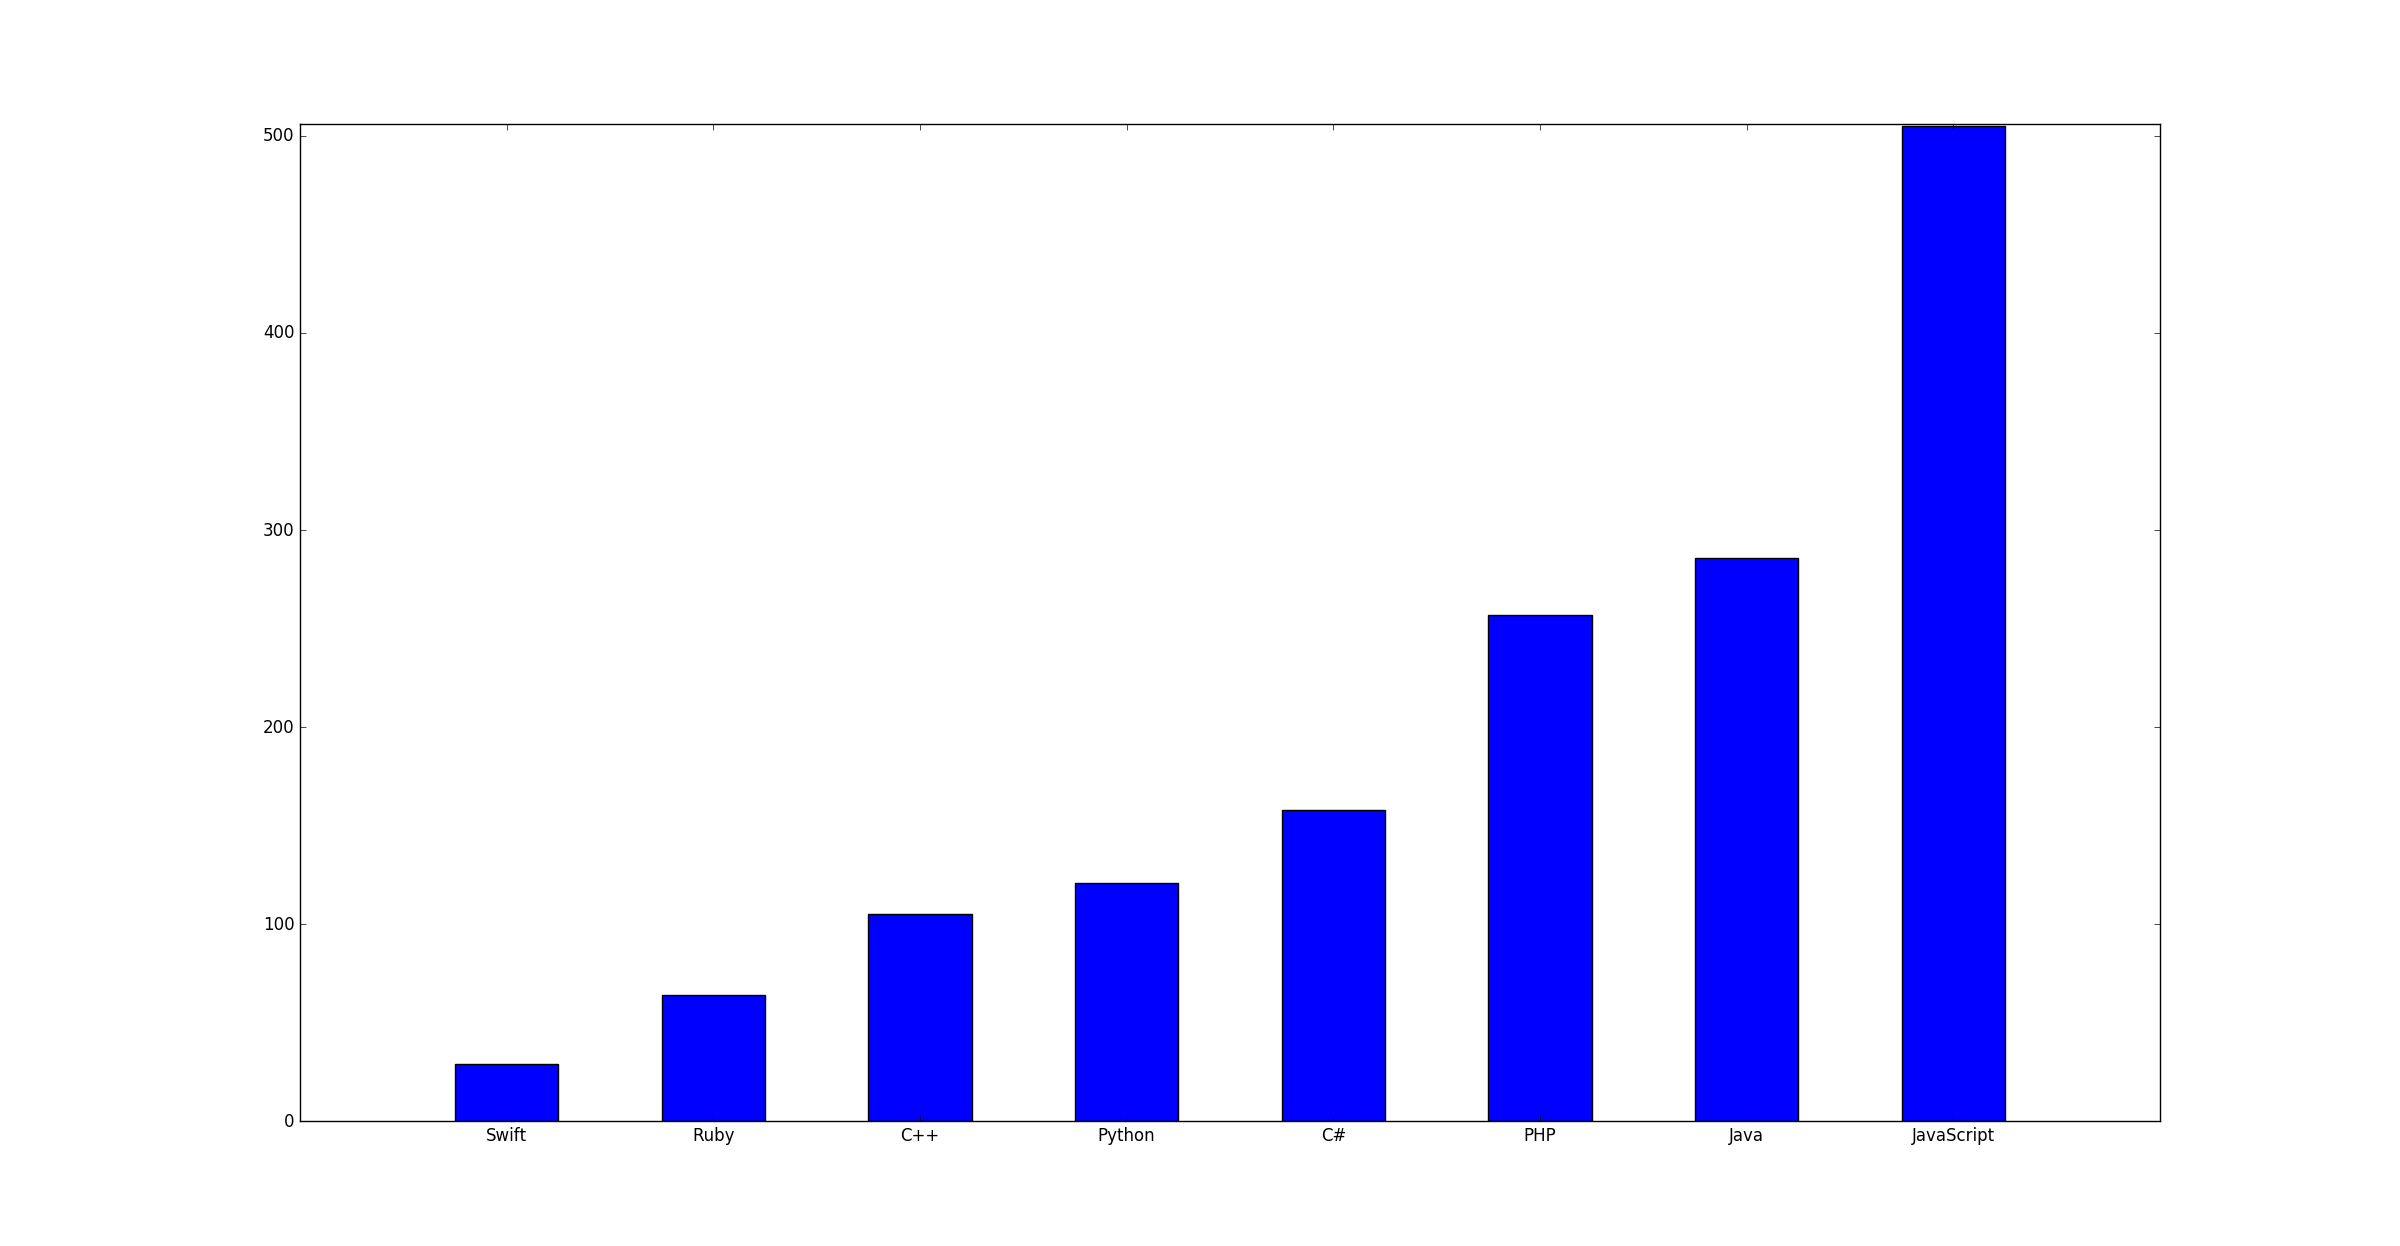
\includegraphics[width=1.1\textwidth]{pictures/minsk_job_tutby.png}
\end{center}
\end{frame}
% ******************************************************

%-------------------------------------------------------
\subsection{Indentation is very important!}
%-------------------------------------------------------



% ********************** Slide 14 **********************
%\begin{frame}[fragile]{Introduction}{Indentation is very important!}
%-------------------------------------------------------
	
%\begin{block}{Indentation}
	
%\begin{lstlisting}[language=Python, tabsize=4, showspaces=true, showtabs=true]
%if True:
%    print("True")
%else:
%    print("False")
%
%if True:
%	print("True")
%    print("Error")
%
%if True:
%    print("True")
%  print("Error")
%\end{lstlisting}
%
%\end{block}	
%	
%\end{frame}


%-------------------------------------------------------
\begin{frame}{Introduction}{Questions?}
%-------------------------------------------------------
	\large Questions?
	\begin{center}
		
		\begin{block}{Contacts}
			\begin{itemize}
				\item Email:    buzuma.leha@gmail.com
				\item Facebook: aleksei.buzuma
			\end{itemize}
		\end{block}
		
	\end{center}
\end{frame}

\end{document}